\section{The instrument was not the same across ecosystems}
\label{sec:instrument}

Each non-Python ecosystem drives CodeCarbon through its own Python bridge. The
campaign shipped five such bridges, and they were configured four different ways.
Table~\ref{tab:instrument} reports what each stack actually used, read from
source.

\begin{table}[t]
\centering
\caption{Instrument configuration per ecosystem, read from the source of each
bridge. Two CodeCarbon major versions, two tracking modes and two sampling
intervals were in use simultaneously.}
\label{tab:instrument}
\small
\begin{tabular}{llllr}
\toprule
Ecosystem & CodeCarbon & Tracking mode & \code{measure\_power\_secs} & Host share \\
\midrule
Python/PyTorch    & 2.8.4 & machine & 15 (default) & \SI{63}{\percent} \\
Python/TensorFlow & 2.8.4 & machine & 15 (default) & \SI{69}{\percent} \\
Python/JAX        & 2.8.4 & machine & 1            & \SI{63}{\percent} \\
Rust/tch          & 2.8.4 & machine & 1            & \SI{63}{\percent} \\
R/torch           & 2.8.4 & \textbf{process} & 1   & \SI{31}{\percent} \\
C++/LibTorch      & 3.0.4 & machine & 15 (default) & \SI{42}{\percent} \\
Java/DL4J         & 3.0.4 & machine & 15 (default) & \SI{40}{\percent} \\
MATLAB/DLT        & 3.0.4 & machine & 15 (default) & \SI{55}{\percent} \\
\bottomrule
\end{tabular}
\end{table}

\subsection{Two thirds of the reported energy is a function of wall-clock time}

The difference between CodeCarbon 2.8.x and 3.0.x is not cosmetic. Where RAPL is
unavailable, 2.8.x substitutes a hardcoded constant for CPU power
(\(\SI{85}{\watt}\times 0.5 = \SI{42.5}{\watt}\)), and models RAM power as
\SI{0.375}{\watt\per\gibi\byte} of \emph{installed} memory --- on this server,
\SI{503}{\gibi\byte}, giving a constant \SI{188.84}{\watt} regardless of use.

For the four stacks on 2.8.4 in machine mode, the identity
\[
\text{cpu\_energy} + \text{ram\_energy} = \SI{231.3}{\watt}\times \text{duration}
\]
holds to within \SI{0.5}{\percent}. Roughly two thirds of their reported energy
is therefore a deterministic linear function of wall-clock time, computed from a
constant that depends on how much memory is physically installed in the machine.
The 3.0.x stacks carry about \SI{107}{\watt} of modelled host power instead, and
R --- the only stack in process mode --- carries almost none: its RAM energy
share is \SI{0.03}{\percent} against roughly \SI{50}{\percent} elsewhere.

Comparing raw \code{energy\_consumed} across these stacks therefore compares
instrument configurations at least as much as it compares ecosystems.

\subsection{The CodeCarbon version was an ambient property of the shell}

The Rust bridge launched its measurement daemon with \code{Command::new("python3")}
--- the first interpreter on \code{PATH}. Which CodeCarbon version measured that
ecosystem was thus a property of the shell that happened to start the run, not a
decision of the experiment. This is the mechanism by which one campaign came to
mix CodeCarbon 2.8.4 and 3.0.4.

\subsection{The bridge was not synchronised with the workload}

Of the three daemon-style bridges, one wrote \code{START} into the daemon's stdin
and began computing immediately, without waiting for the tracker to exist.
CodeCarbon takes seconds to initialise, so the tracked window did not cover the
work it was meant to measure. Measured on an RTX 3090 for one epoch of
ResNet-18/CIFAR-100:

\begin{center}
\small
\begin{tabular}{lrr}
\toprule
Block & Unsynchronised & Synchronised \\
\midrule
Inference & \SI{0}{\joule} (on real GPU work) & \SI{97}{\joule} \\
Training  & \SI{861}{\joule} & \SI{1127}{\joule} \\
\bottomrule
\end{tabular}
\end{center}

\noindent
The inference block recorded nothing at all; the training block was
underestimated by \SI{24}{\percent}. The other two bridges were synchronous: the
Java bridge waits on a ready latch, and the C++ bridge embeds the interpreter and
is synchronous by construction. This defect is therefore not a property of the
approach but of one implementation of it --- which is precisely why it survived.

\begin{figure}[t]
\centering
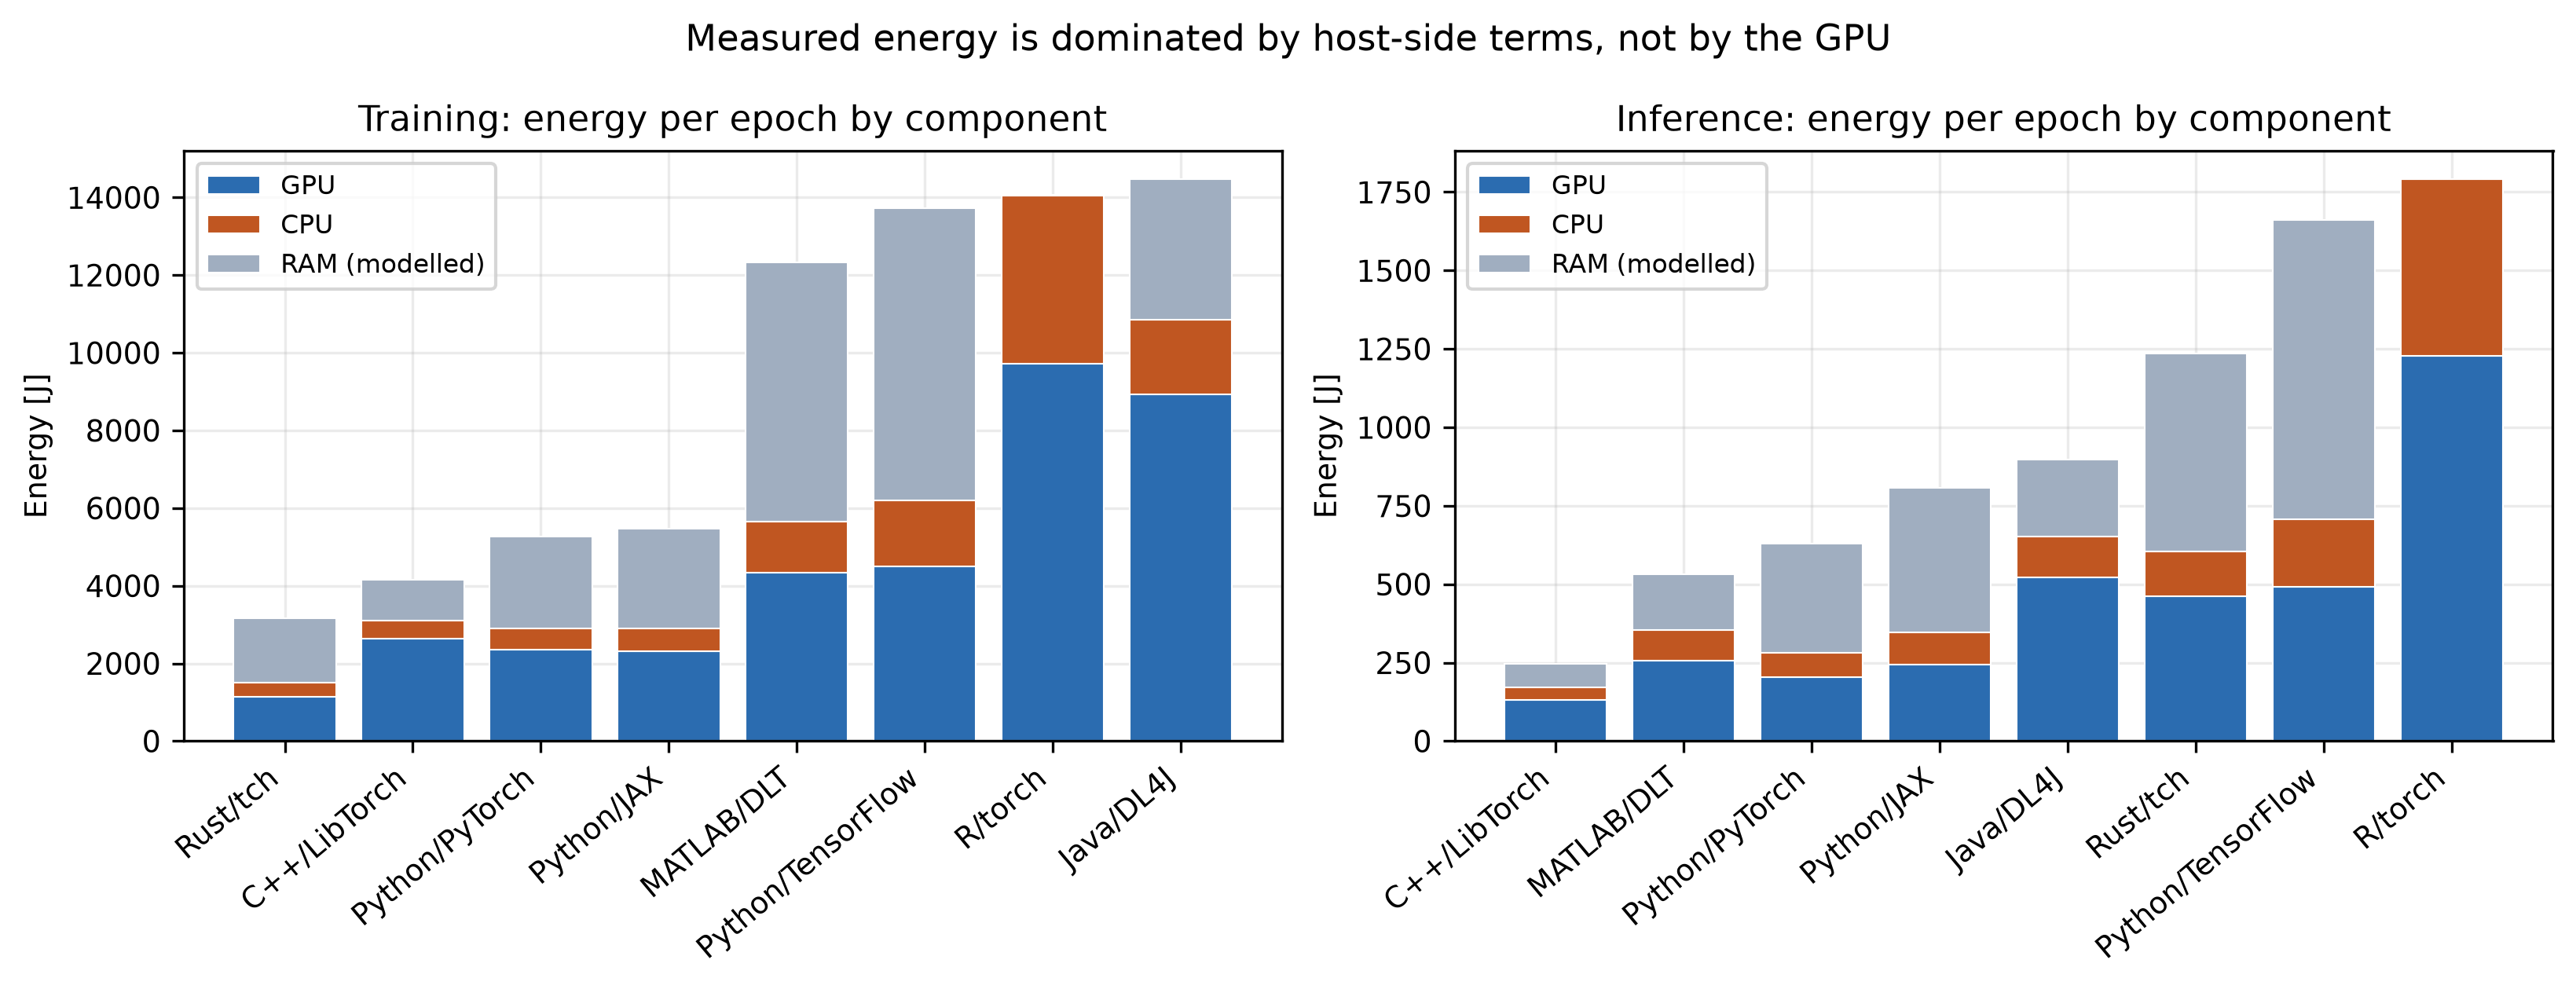
\includegraphics[width=\linewidth]{figures/fig_component_breakdown.png}
\caption{Energy per epoch split into GPU, CPU and modelled RAM. The RAM term is
not measured: for the CodeCarbon 2.8.x stacks it is a constant
\SI{188.84}{\watt} derived from \emph{installed} memory, so it grows only with
wall-clock time. It is the largest single component for four of the eight
ecosystems.}
\label{fig:components}
\end{figure}

\subsection{The workload does not load the accelerator}

Mean GPU power derived from the energy counter ranges from \SI{83}{\watt} to
\SI{197}{\watt} against a \SI{350}{\watt} board limit, and never approaches the
limit in any configuration. Between \SI{30}{\percent} and \SI{69}{\percent} of
the measured energy is GPU energy; the remainder is host-side. At that
utilisation the campaign measures data loading and dispatch more than it measures
deep learning (Figure~\ref{fig:gpuload}).

\begin{figure}[t]
\centering
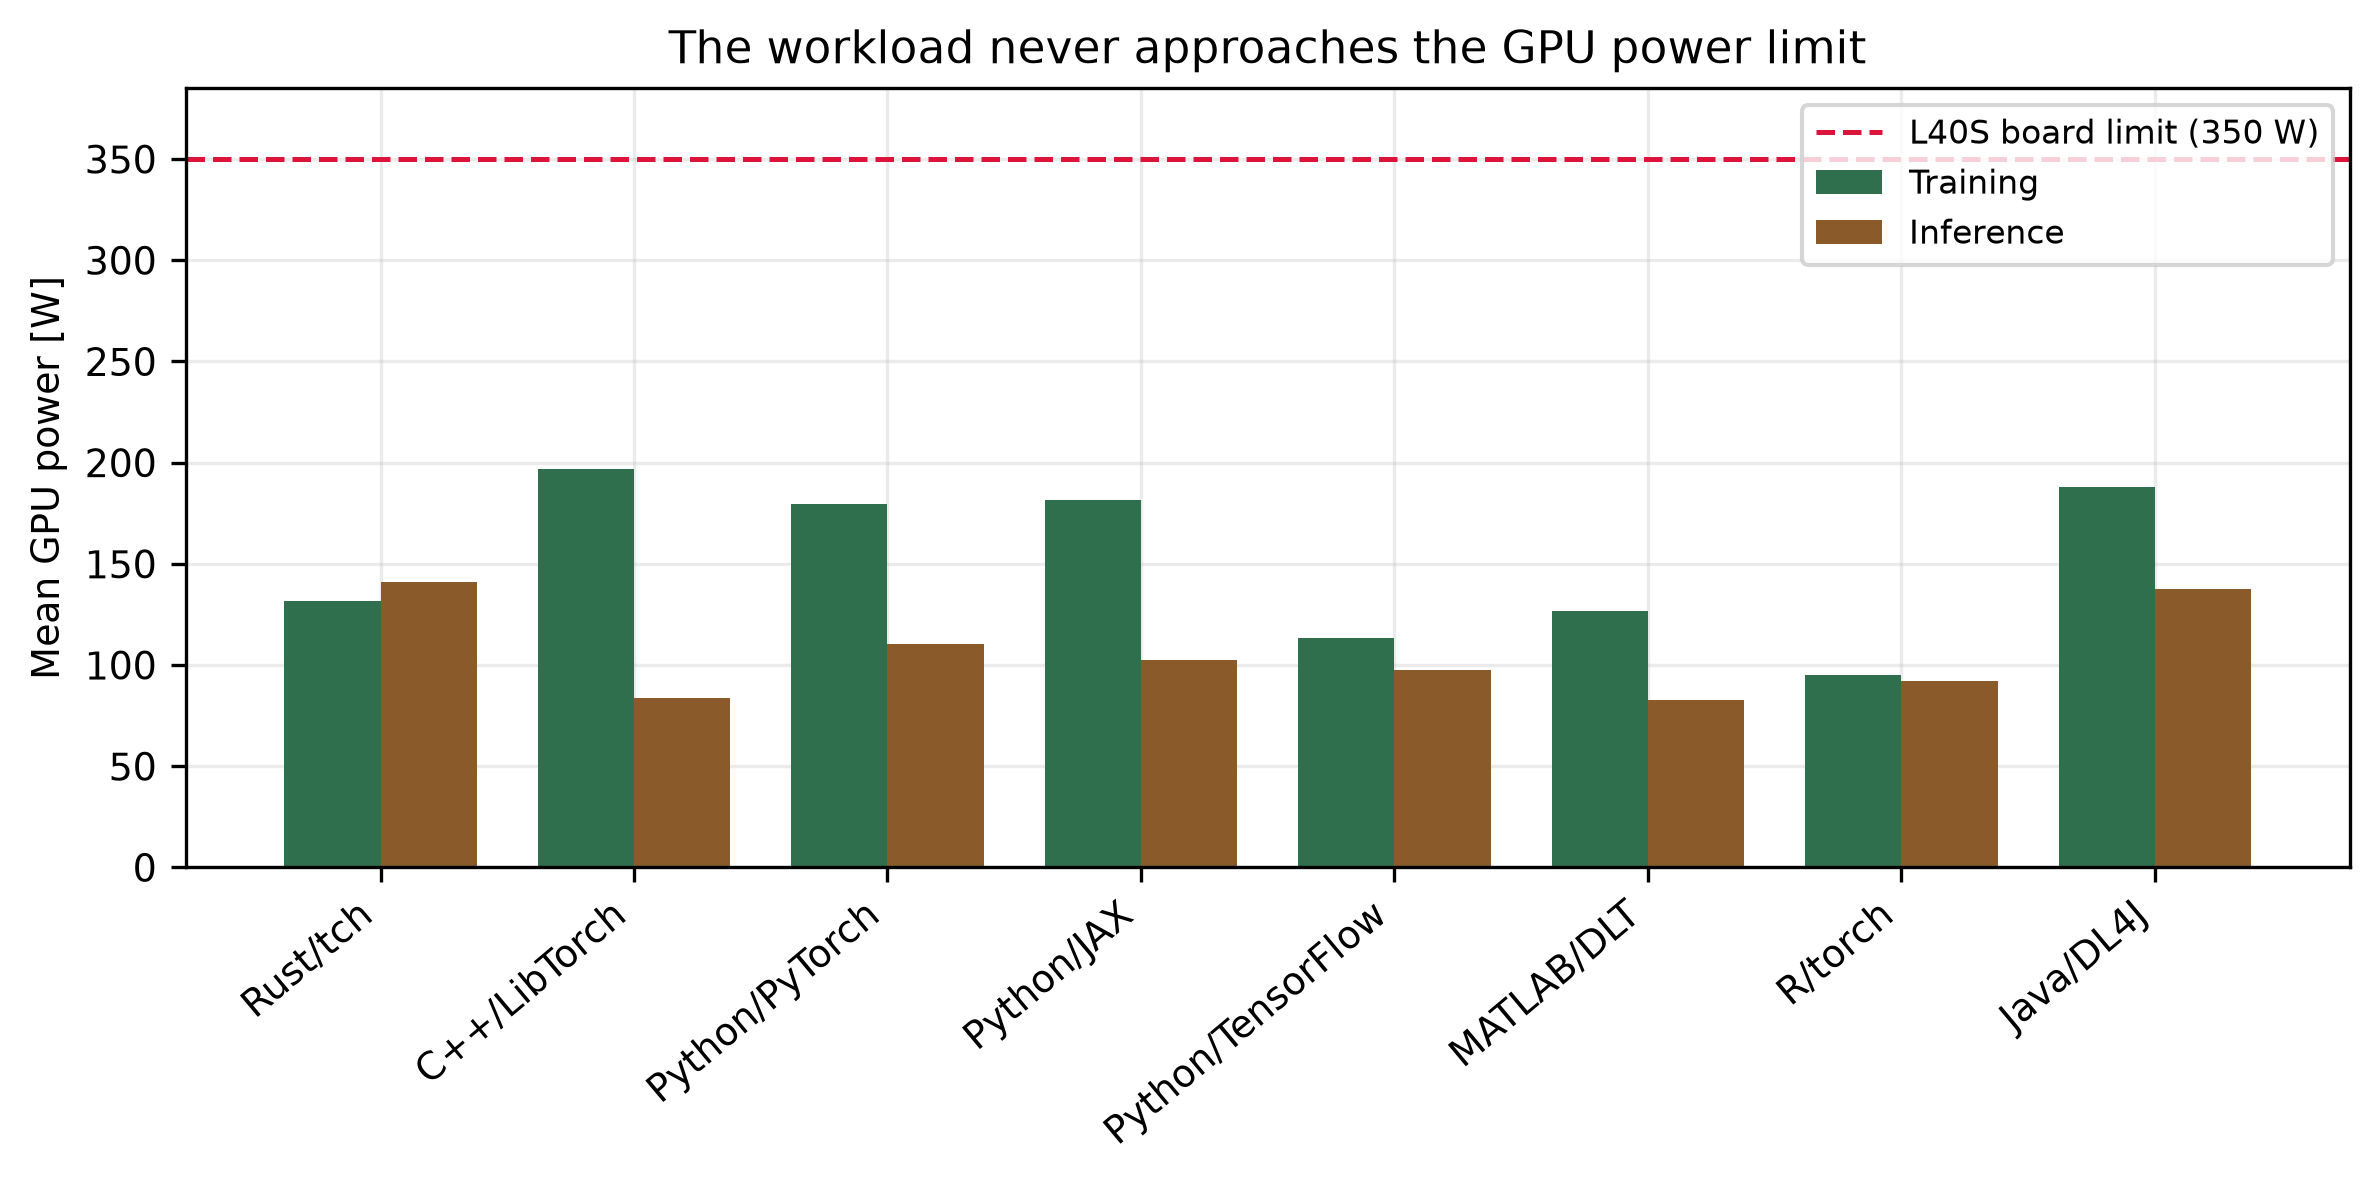
\includegraphics[width=0.72\linewidth]{figures/fig_gpu_load.png}
\caption{Mean GPU power per ecosystem and phase, against the board limit of the
measurement device. No configuration approaches the limit in either phase.}
\label{fig:gpuload}
\end{figure}
